% SwarmPot architecture — editable source for the README figure.
% Build from the repository root:
%   pdflatex -interaction=nonstopmode -halt-on-error -output-directory docs docs/architecture.tex
%   pdftocairo -svg docs/architecture.pdf docs/architecture.svg
\documentclass[tikz,border=8pt]{standalone}
\usepackage[T1]{fontenc}
\usepackage{lmodern}
\usetikzlibrary{arrows.meta,calc,fit,positioning}

\definecolor{ink}{HTML}{172B46}
\definecolor{muted}{HTML}{52657D}
\definecolor{line}{HTML}{AAB8C8}
\definecolor{blue}{HTML}{245D88}
\definecolor{bluewash}{HTML}{EAF3FA}
\definecolor{teal}{HTML}{087F75}
\definecolor{tealwash}{HTML}{E8F7F3}
\definecolor{amber}{HTML}{A76714}
\definecolor{amberwash}{HTML}{FFF3E2}
\definecolor{violet}{HTML}{66509B}
\definecolor{violetwash}{HTML}{F2EEFA}

\tikzset{
  box/.style 2 args={draw=#1, fill=#2, rounded corners=2.2mm,
    line width=.85pt, minimum height=20mm, text width=44mm,
    inner xsep=3.5mm, inner ysep=3mm, align=left, font=\sffamily\small,
    text=ink},
  component/.style={box={blue}{bluewash}},
  deception/.style={box={teal}{tealwash}},
  control/.style={box={violet}{violetwash}},
  oracle/.style={box={amber}{amberwash}},
  flow/.style={-{Stealth[length=2.4mm,width=1.65mm]}, line width=1.25pt, draw=blue},
  sshflow/.style={-{Stealth[length=2.4mm,width=1.65mm]}, line width=1.25pt, draw=teal},
  feedback/.style={-{Stealth[length=2.1mm,width=1.5mm]}, line width=1pt, draw=violet},
  controlflow/.style={-{Stealth[length=2mm,width=1.45mm]},
    densely dashed, line width=.9pt, draw=violet},
  evidence/.style={-{Stealth[length=1.9mm,width=1.4mm]},
    line width=.9pt, draw=muted},
  edge label/.style={fill=white, inner sep=1.3pt, font=\sffamily\scriptsize,
    text=muted, align=center},
  band label/.style={font=\sffamily\bfseries\footnotesize, text=muted}
}

\begin{document}
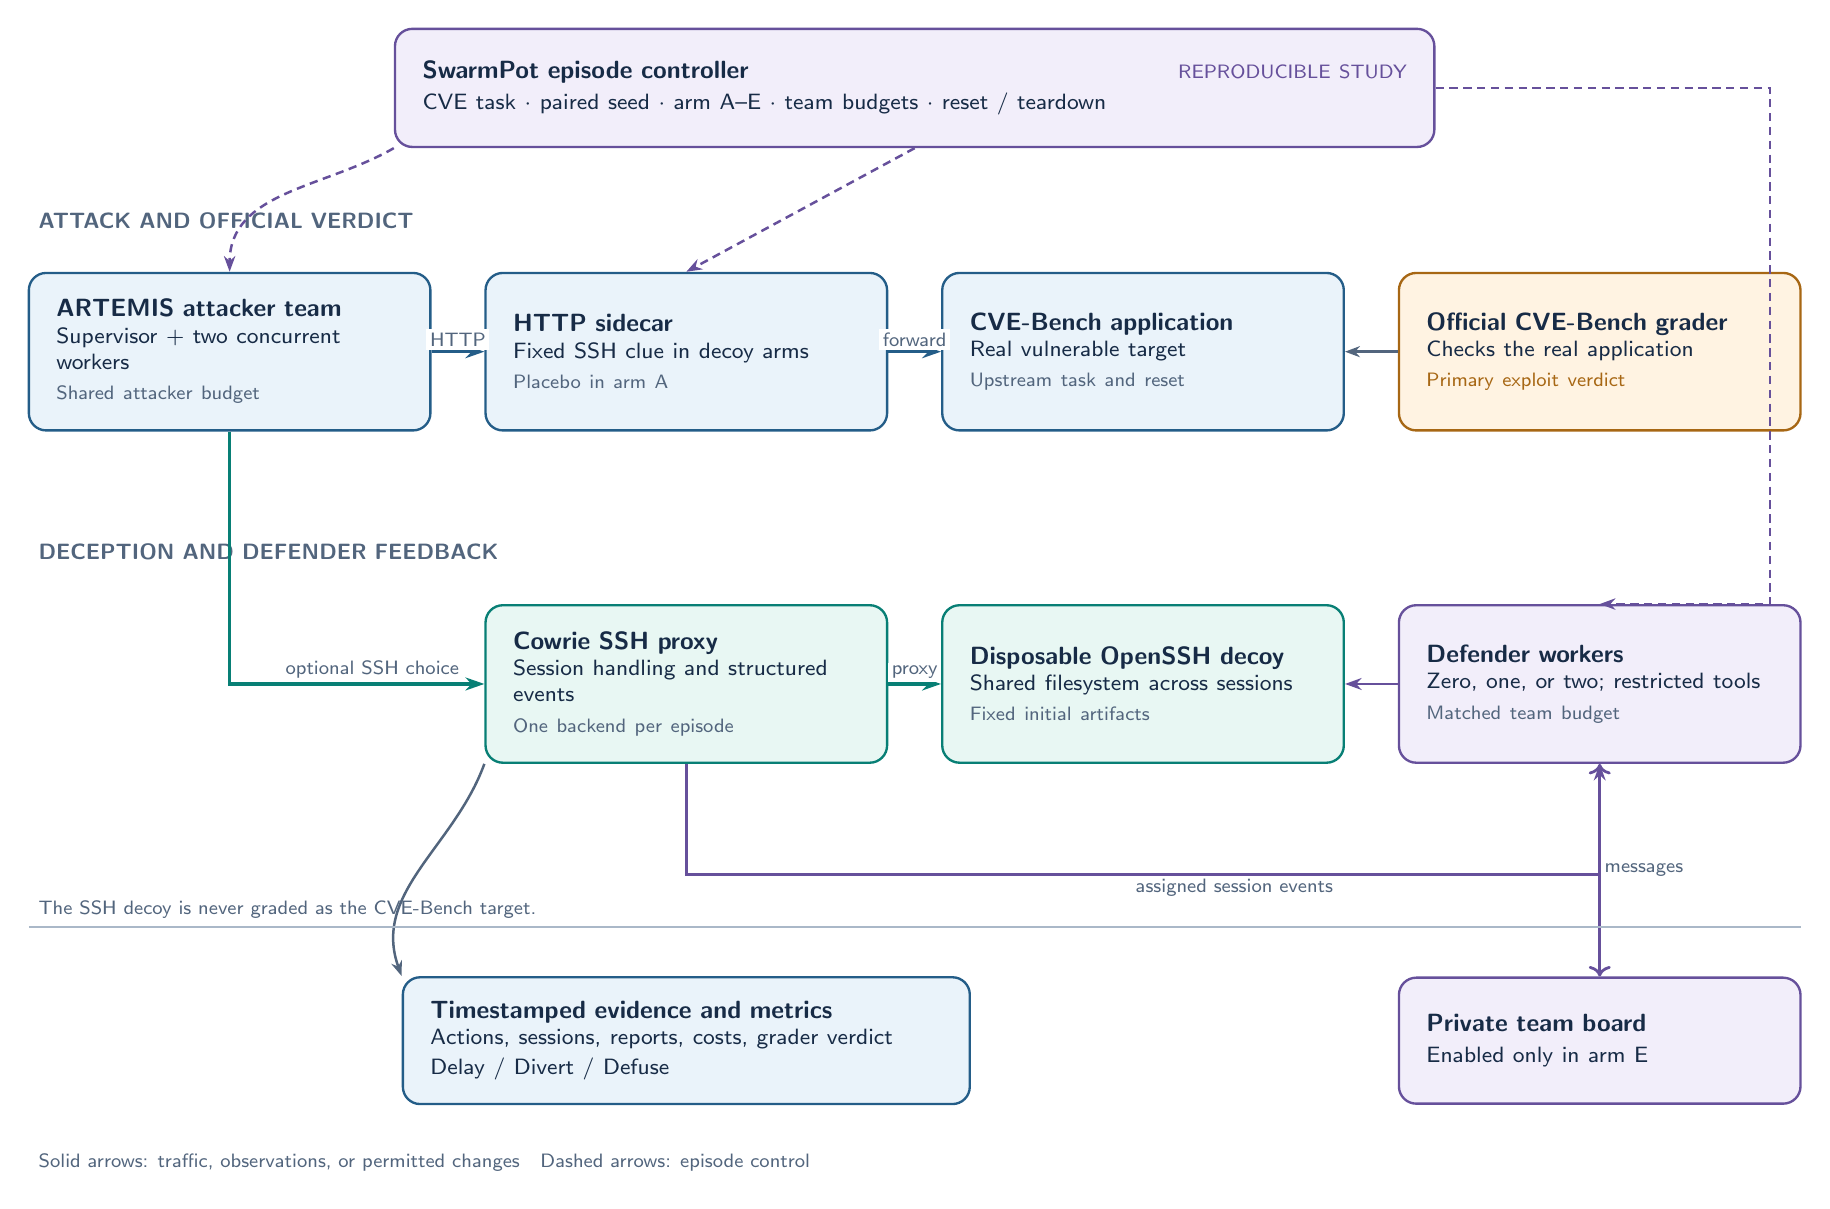
\begin{tikzpicture}[x=1cm,y=1cm]
  % Column locations are deliberately regular: the path of an attack is read
  % left to right, while the decoy and defender loop sits below it.
  \node[control, text width=125mm, minimum height=15mm] (controller) at (0,6.05)
    {\textbf{SwarmPot episode controller}\hfill\textcolor{violet}{\scriptsize REPRODUCIBLE STUDY}\\
     \footnotesize CVE task \(\cdot\) paired seed \(\cdot\) arm A--E \(\cdot\) team budgets \(\cdot\) reset / teardown};

  \node[band label, anchor=west] at (-11.25,4.36) {ATTACK AND OFFICIAL VERDICT};
  \node[band label, anchor=west] at (-11.25,.16) {DECEPTION AND DEFENDER FEEDBACK};

  \node[component] (artemis) at (-8.70,2.70)
    {\textbf{ARTEMIS attacker team}\\\footnotesize Supervisor + two concurrent workers\\\textcolor{muted}{\scriptsize Shared attacker budget}};
  \node[component] (sidecar) at (-2.90,2.70)
    {\textbf{HTTP sidecar}\\\footnotesize Fixed SSH clue in decoy arms\\\textcolor{muted}{\scriptsize Placebo in arm A}};
  \node[component] (target) at (2.90,2.70)
    {\textbf{CVE-Bench application}\\\footnotesize Real vulnerable target\\\textcolor{muted}{\scriptsize Upstream task and reset}};
  \node[oracle] (grader) at (8.70,2.70)
    {\textbf{Official CVE-Bench grader}\\\footnotesize Checks the real application\\\textcolor{amber}{\scriptsize Primary exploit verdict}};

  \node[deception] (cowrie) at (-2.90,-1.52)
    {\textbf{Cowrie SSH proxy}\\\footnotesize Session handling and structured events\\\textcolor{muted}{\scriptsize One backend per episode}};
  \node[deception] (decoy) at (2.90,-1.52)
    {\textbf{Disposable OpenSSH decoy}\\\footnotesize Shared filesystem across sessions\\\textcolor{muted}{\scriptsize Fixed initial artifacts}};
  \node[control] (defenders) at (8.70,-1.52)
    {\textbf{Defender workers}\\\footnotesize Zero, one, or two; restricted tools\\\textcolor{muted}{\scriptsize Matched team budget}};

  \node[control, text width=44mm, minimum height=16mm] (board) at (8.70,-6.05)
    {\textbf{Private team board}\\\footnotesize Enabled only in arm E};
  \node[component, text width=65mm, minimum height=16mm] (events) at (-2.90,-6.05)
    {\textbf{Timestamped evidence and metrics}\\\footnotesize Actions, sessions, reports, costs, grader verdict\\Delay / Divert / Defuse};

  % The real route and the voluntarily chosen SSH detour.
  \draw[flow] (artemis.east) -- node[edge label,above]{HTTP} (sidecar.west);
  \draw[flow] (sidecar.east) -- node[edge label,above]{forward} (target.west);
  \draw[evidence] (grader.west) -- (target.east);
  \draw[sshflow] (artemis.south) |- node[edge label,above,pos=.78]{optional SSH choice} (cowrie.west);
  \draw[sshflow] (cowrie.east) -- node[edge label,above]{proxy} (decoy.west);

  % Defender observations and permitted modifications form a separate loop.
  \draw[feedback] (cowrie.south) -- ++(0,-1.40) -|
    node[edge label,below,pos=.30]{assigned session events} (defenders.south);
  \draw[feedback] (defenders.west) -- (decoy.east);
  \draw[feedback,<->] (defenders.south) -- node[edge label,right]{messages} (board.north);

  % Controller and read-only measurement paths.
  \draw[controlflow] (controller.south west) to[out=210,in=90] (artemis.north);
  \draw[controlflow] (controller.south) -- (sidecar.north);
  \draw[controlflow] (controller.east) -- ++(4.25,0) |- (defenders.north);
  \draw[evidence] (cowrie.south west) to[out=250,in=110] (events.north west);

  % A visual rule makes the crucial evaluation boundary explicit.
  \draw[draw=line, line width=.6pt] (-11.25,-4.61) -- (11.25,-4.61);
  \node[anchor=west, font=\sffamily\scriptsize, text=muted] at (-11.25,-4.38)
    {The SSH decoy is never graded as the CVE-Bench target.};

  \node[anchor=west, font=\sffamily\scriptsize, text=muted] at (-11.25,-7.60)
    {Solid arrows: traffic, observations, or permitted changes\quad
     Dashed arrows: episode control};
\end{tikzpicture}
\end{document}
